\label{chapter:testsBdd}
\gab{Destacar aqui duas finalidades - 1 .testar o próprio simulador. 2. Implementar testes automatizados do comportamento de sistemas  utilizam o simulador}

A fim de fazer a verificação e validação do simulador HMR Sim, foi proposto utilizar o Behavior Driven Development. Dessa forma foi sugerido um framework de testes para ajudar no processo. O framework é composto por \del{uma estrutura de pastas, composta pelas especificações das missões na linguagem Gherkin, dos testes dessas missões e por }um conjunto de métodos desenvolvidos para auxiliar na criação e nas assertivas dos cenários.

\section{Estruturação dos Testes}
\label{sec:estruturacaoTestes}
\begin{figure}
\centering
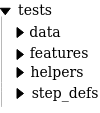
\includegraphics[scale=0.8]{imagens/estrutura_pasta.png}
\caption{Estrutura de pasta dos testes.} 
\label{fig:estruturaPasta}
\end{figure}

A parte de teste é dividida em quatro pastas:
\begin{itemize}
    \item \textbf{features}: Contém a descrição dos cenários e passos de cada funcionalidade. Cada funcionalidade está descrita em um arquivo .feature, que faz uso da linguagem Gherkin. Os arquivos das Features são estruturados da seguinte forma:
    \begin{itemize}
        \item Os passos Given são responsáveis por fazer a montagem do cenário, por exemplo, instanciar uma simulação, associar um mapa à simulação, adicionar sistemas, criar POIs (pontos de interesse), criar caminhos, adicionar componentes ao robô.
        \item Os passos When são responsáveis por executar a simulação, chamando o método run da simulação.
        \item Os passos Then são responsáveis por fazer as assertivas, verificando se a simulação fez o que era esperado.
    \end{itemize}
    \item \textbf{step\_defs}: Os arquivos dessa pasta possuem a montagem dos passos da simulação, a execução da simulação e as assertivas. Cada arquivo da pasta step\_defs é relacionado com um arquivo .feature da pasta features e todos os passos presentes no .feature devem estar presentes também no arquivo de testes, conforme mostra a figura \ref{fig:singleStaticRobotF} e a figura \ref{fig:singleStaticRobotT}. 
No início dos arquivos ocorre a instanciação da simulação e dos helpers (ScenarioCreationHelper e AssertionHelper), que serão usados nos passos given, when e then.
    \item \textbf{helpers}: A pasta possui duas classes de métodos auxiliares. A primeira classe, a ScenarioCreationHelper, possui métodos para auxiliar na criação dos cenário, sendo alguns desses métodos: add\_component (adiciona um componente em uma entidade), create\_path (cria um caminho que parte de uma entidade e passa por diferentes pontos no mapa), add\_goto\_position\_event (adiciona um evento na event store para que o robô se movimente até uma determinada posição), add\_poi (adiciona um ponto de interesse na mapa). A segunda classe, a AssertionHelper, possui métodos para auxiliar nas assertivas, contendo mensagens de erros mais completas. Sendo alguns desses métodos: have\_collided (verifica se uma entidade colidiu com outra entidade), is\_in\_poi (verifica se o centro de uma entidade está posicionado em um ponto), approximated (verifica se um robô X se aproximou de uma entidade Y).
    
\begin{figure}
\centering
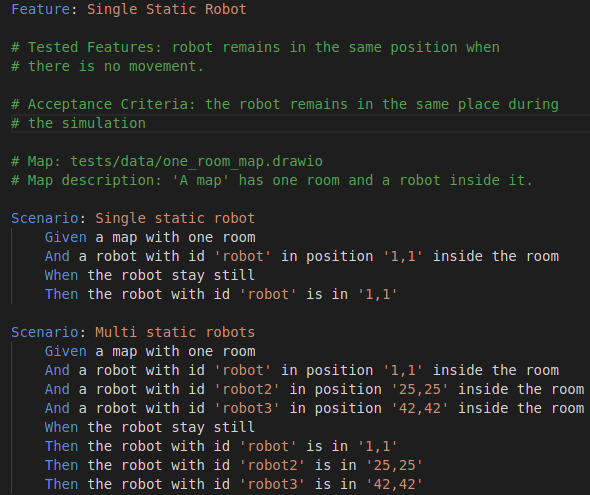
\includegraphics[scale=0.5]{imagens/single_static_robot_feature.png}
\caption{Arquivo single\_static\_robot.feature.} 
\label{fig:singleStaticRobotT}
\end{figure}

\begin{figure}
\centering
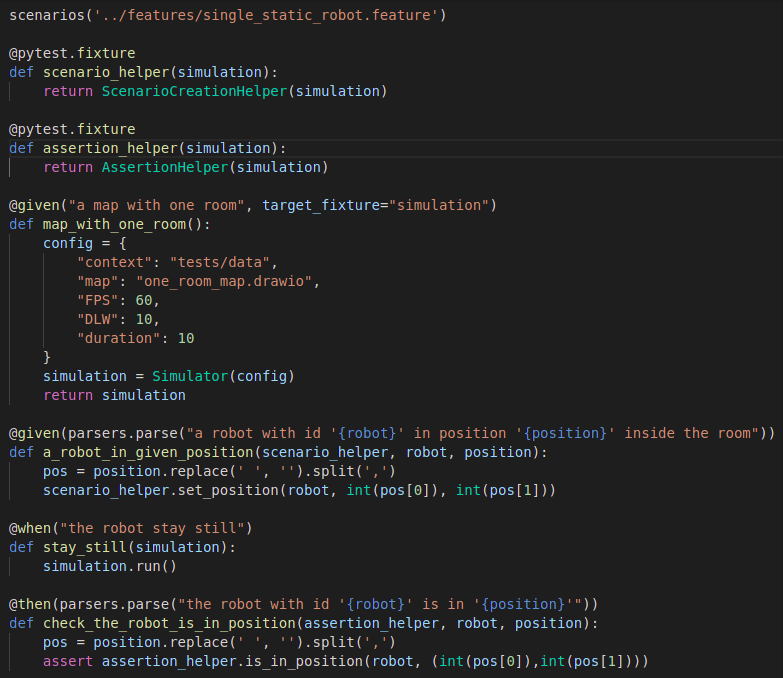
\includegraphics[scale=0.5]{imagens/test_single_static_robot.png}
\caption{Arquivo de teste test\_single\_static\_robot.py.} 
\label{fig:singleStaticRobotF}
\end{figure}
    
    \item \textbf{data}: Possui os mapas necessários para a criação de uma simulação. Os mapas são feitos utilizando a ferramenta draw io.

\end{itemize}
\section{Capacidades e Limitações}
\label{sec:limitacoesTeste}
\gab{Mover a discussão sobre as limitações para o final do capítulo. Primeiro o leitor deve ter uma idéia do que é capaz para depois saber as limitações.}
A princípio, é possível verificar:
\begin{itemize}
    \item Posições finais de entidades;
    \item Informações salvas em componentes que são capturadas durante a execução dos sistemas.
\end{itemize}

Não é possível verificar:
\begin{itemize}
    \item Informações que não fazem parte do estado final  da simulação, a não ser que essa informação tenha sido gerada por um dos sistemas e tenha sido guardada em algum componente que possa ser acessado ao término da execução;
    \item Informações que mudam a cada vez que a simulação é executada, ou seja, não é possível testar informações que não são possíveis de se reproduzir.
\end{itemize}

Nos testes são feitos os seguintes tipos de verificações e existem as seguintes limitações:
\begin{itemize}
    \item \textbf{Robot Displacement}: é verificado se um robô foi até a posição requisitada (posição final do robô), mas não verifica o caminho que ele percorreu.

    \item \textbf{Scripted Commands}: são verificadas se determinadas entidades estão na posição ou ponto de interesse (POI) correto. Um dos cenários, testa se um medicamento (pickable) foi deixado em uma determinada posição. No entanto, só se verifica a posição final dele. Para verificar posições intermediárias é necessário guardar em um componente as informações dos locais que o robô deixou o pickable.

    \item \textbf{Collision}: é verificado se um robô colidiu com outra entidade, para isso é testado se o identificador da entidade colidida está presente na lista de colisões do robô, guardada no componente CollisionHistory. Uma limitação dessa abordagem é que só é guardado a última colisão entre o robô e uma determinada entidade.

    \item \textbf{Seer}: é possível acessar as mensagens geradas pelo Seer, mas é necessário guardá-las em um componente ou em arquivo para depois acessar essas mensagens e testá-las. No entanto, é trabalhoso testar se todos os logs estão no formato esperado, e se a formatação das mensagens muda, é preciso mudar as assertivas. Por conta disso, o teste do Seer verifica apenas se o arquivo gerado possui pelo menos uma linha no formato json, e se essa primeira linha possui uma chave com o nome “timestamp”.
    
    \item \textbf{Camera}: é possível verificar se uma ou mais entidades foram detectadas por um robô que possui o componente Camera. No entanto, uma das limitações é que a câmera guarda apenas uma detecção de um alvo (a última adicionada), por exemplo, se detectar uma pessoa duas vezes, guarda apenas a última detecção.

    \item \textbf{Approximation}: é verificado se o robô se movimentou até a pessoa detectada, sendo essa informação guardada em um componente do tipo ApproximationHistory. No momento não é possível fazer duas aproximações porque a Câmera é removida quando a primeira aproximação ocorre e o ApproximationHistory só guarda informações de uma aproximação.
\end{itemize}

Para verificar passos intermediários, por exemplo, verificar os pontos que o robô parou durante a simulação, é necessário guardar a informação em uma lista para depois acessá-la na hora de fazer a verificação.

Uma outra limitação está presente nos métodos de assertivas (tests/helpers/AssertionHelper.py): A maioria dos métodos verifica apenas o caso verdadeiro, caso contrário lança um erro (raise AssertionError). Então para verificar os casos falsos seria necessário fazer modificações nos métodos ou criar novos.

\section{Criando uma Feature utilizando o HMR Sim e princípios do BDD}
\label{sec:featureBDD}
Como parte da validação do simulador, foi feito um sistema a partir do zero, desde a criação dos cenários e testes até a implementação de novos mapas, componentes e sistemas.

Utilizando o Sistema de Aproximação proposto, o robô é capaz de percorrer um caminho procurando uma pessoa, para isso utiliza um componente do tipo câmera, e se essa pessoa estiver no campo de visão da câmera, ele se aproxima dela. 

\subsection{Sistema de Detecção e de Aproximação}
\label{sec:sistemaAprox}
A lógica do sistema de aproximação foi dividida em duas partes. A primeira parte é a responsável por detectar uma entidade solicitada utilizando o CameraProcessor. Já a segunda parte é feita através do sistema de aproximação (ApproximationDESProcessor) e é a responsável por navegar até a pessoa que foi detectada.

A implementação do sistema da câmera foi feita utilizando um sistema já implementado anteriormente, o Sensor System.

A cada iteração, o SensorSystem verifica se existem entidades próximas do sensor. Neste caso, o sensor que será passado como parâmetro é um componente do tipo câmera. Se existirem entidades próximas, o SensorSystem envia um evento contendo um vetor de entidades próximas  para o reply chanel da câmera. Essa etapa é feita utilizando um sistema Publisher/Subscriber, no qual o SensorSystem (Publisher) envia informações 
para uma câmera que fica esperando por essas informações (Subscriber).

Nessa parte entra um segundo sistema, o CameraProcessor, que fica esperando receber essas informações que foram enviadas para o reply chanel da câmera. Esse processador recebe como parâmetro uma câmera e o identificador da entidade que será detectada. Assim que recebe as informações de entidades próximas, o processador compara se uma dessas entidades detectadas era o alvo. Se a entidade detectada for igual ao alvo,essa informação é adicionada à lista de entidades detectadas da câmera e também é enviado um evento avisando sobre a detecção.

Para que o sistema de detecção funcione é necessário:
\begin{itemize}
    \item Adicionar ao robô um componente do tipo Câmera; (colocar o código da função auxiliar);
    \item Iniciar um SensorSystem passando essa câmera como parâmetro e adicionar esse sensor aos DES Systems;
    \item Adicionar um sistema para processar os eventos da câmera.
\end{itemize}

A segunda e última parte do sistema de aproximação é responsável por receber o evento do CameraProcessor que avisa sobre a detecção e a partir disso, o robô se locomove até a entidade detectada. Para fazer a aproximação, o ApproximationDESSystem envia um outro evento do tipo GotoPosEvent que será recebido pelo sistema de navegação, que já foi implementado anteriormente.

Para utilizar esse sistema é necessário:
\begin{itemize}
    \item Adicionar as habilidades de navegação, de detecção de entidades e de aproximação;
    \item Adicionar uma câmera ao robô; 
    \item Adicionar um processador para que o robô procure pela pessoa.
\end{itemize}

\subsection{Criando as funcionalidades de detecção e aproximação utilizando princípios do BDD}
\label{sec:criandoFunc}
O passo inicial antes de implementar as funcionalidades foi a realização dos testes. 

Primeiro foram feitos os testes e a implementação do sistema da Câmera, pois o sistema de aproximação depende dele. Para isso, foram definidos quatro cenários no arquivo camera.feature utilizando a linguagem Gherkin. A figura \ref{fig:cameraFeat} mostra a definição do primeiro cenário.

\begin{figure}
\centering
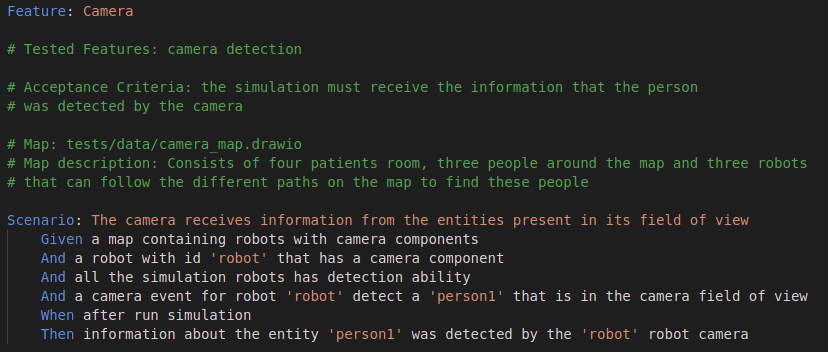
\includegraphics[width=\textwidth]{imagens/cameraFeature.png}
\caption{Definição do primeiro cenário da feature Camera.} 
\label{fig:cameraFeat}
\end{figure}

Depois de descrever os cenários, foi feito um mapa, utilizando o draw io, contendo quartos de pacientes, robôs, pessoas, rotas e pontos de interesse (POIs) para o robô se locomover, conforme mostra a figura \ref{fig:mapaApprox}.

\begin{figure}
\centering
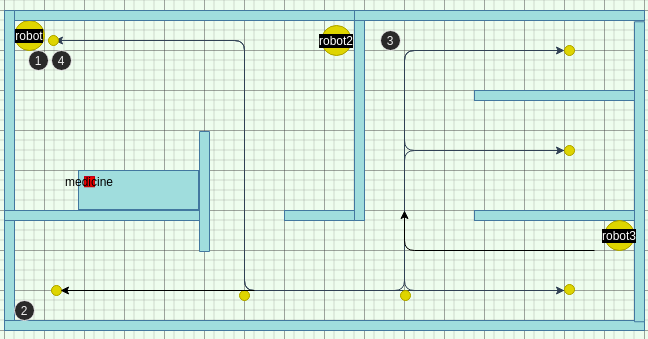
\includegraphics[width=\textwidth]{imagens/mapaApprox.png}
\caption{Mapa dos cenários de detecção e de aproximação.} 
\label{fig:mapaApprox}
\end{figure}

Logo após, foi feita a criação de todos os passos necessários para implementar o cenário da Feature e verificar se tudo ocorreu conforme o esperado, no arquivo test\_camera.py. Nessa etapa é instanciada a simulação e os métodos auxiliares, e também é adicionada a câmera e todos os sistemas necessários, conforme mostra a figura \ref{fig:testCamera}. No entanto, os testes ainda não passam nessa etapa, pois o sistema ainda não foi implementado.

\begin{figure}
\centering
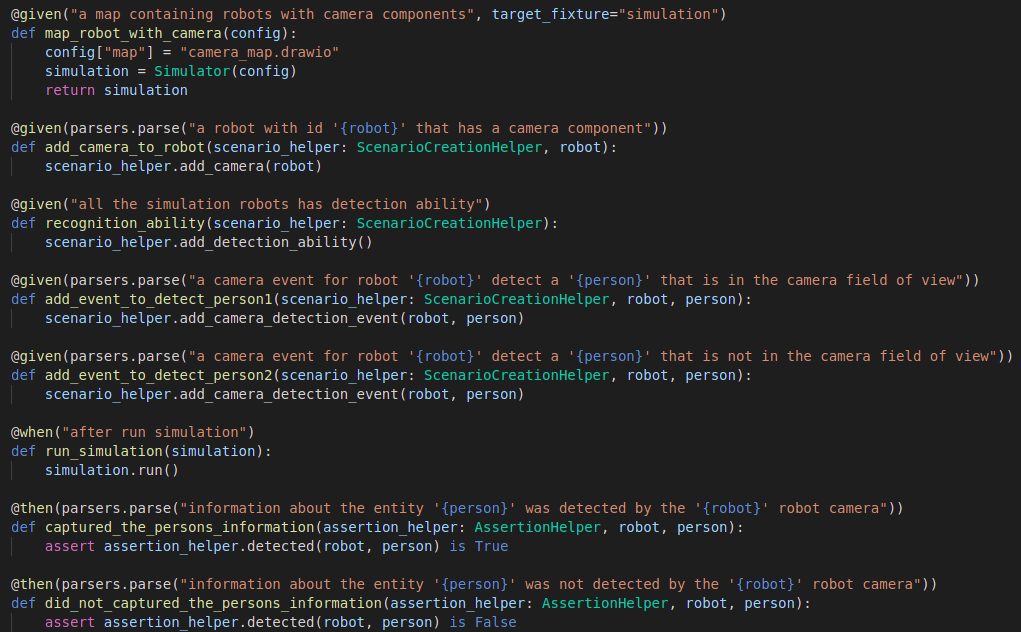
\includegraphics[width=\textwidth]{imagens/testCamera.png}
\caption{Arquivo de teste test\_camera.py.} 
\label{fig:testCamera}
\end{figure}

Em seguida, foi feita a implementação do processador da câmera, o CameraProcessor, que verifica se a câmera detecta um determinado alvo, conforme descrito mais acima. Nessa etapa também é criado um componente do tipo Camera \ref{fig:cameraComp} que herda da classe Component.

\begin{figure}
\centering
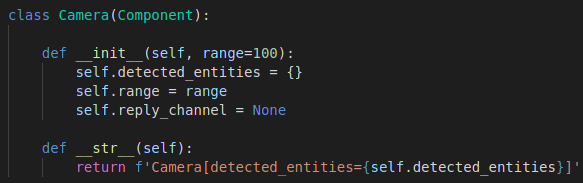
\includegraphics[scale=0.5]{imagens/cameraComp.png}
\caption{Novo componente criado: Camera.} 
\label{fig:cameraComp}
\end{figure}

Retornando aos testes, foi implementado os métodos auxiliares para adicionar o componente de câmera ao robô, para iniciar e adicionar o SensorSystem e para adicionar um processador para receber os eventos de detecção da câmera. Também foi feito um método de assertiva para verificar se ocorreu a detecção.

\begin{figure}
\centering
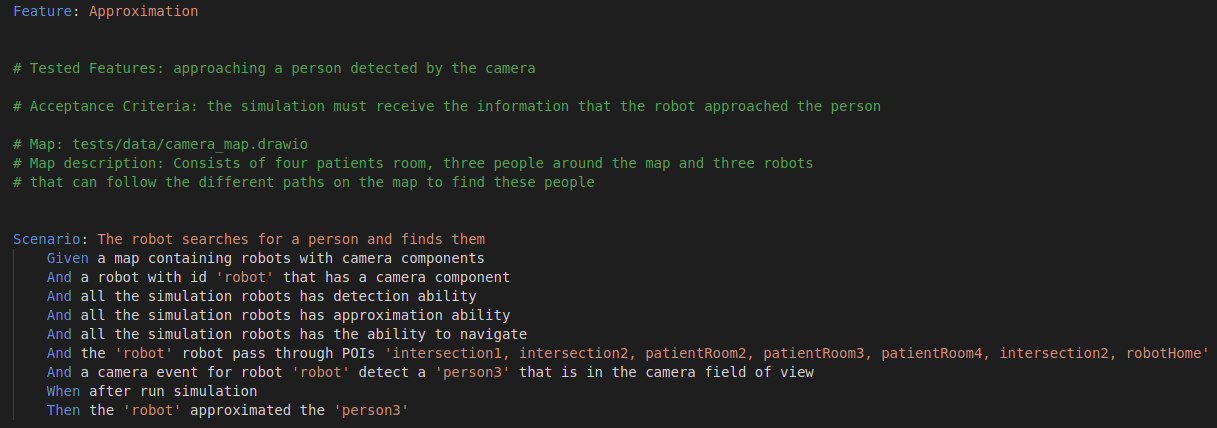
\includegraphics[width=\textwidth]{imagens/approxFeat.png}
\caption{Definição do primeiro cenário da feature Approximation.} 
\label{fig:approxFeat}
\end{figure}

Depois de implementado o sistema de detecção, foi feito o sistema de aproximação, seguindo os mesmos passos descritos acima. Primeiro foram definidos os cenários no arquivo approximation.feature, conforme mostra a figura \ref{fig:approxFeat} e depois foi feita a implementação dos testes no arquivo test\_approximation.py, conforme mostra a figura \ref{fig:Appr1} e a continuação dela \ref{fig:Appr2}. 

\begin{figure}
\centering
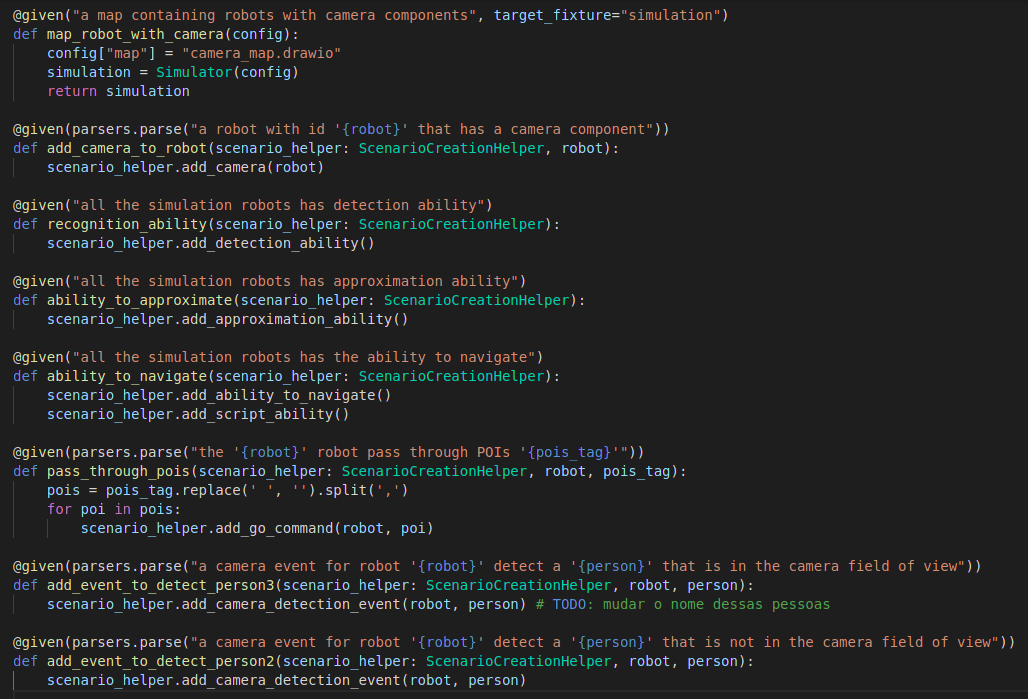
\includegraphics[width=\textwidth]{imagens/Appr1.png}
\caption{Arquivo de teste test\_approximation.py.} 
\label{fig:Appr1}
\end{figure}

\begin{figure}
\centering
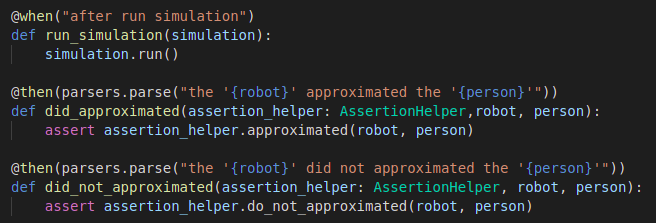
\includegraphics[width=\textwidth]{imagens/Appr2.png}
\caption{Continuação do arquivo de teste test\_approximation.py.} 
\label{fig:Appr2}
\end{figure}

O arquivo de mapa usado é o mesmo do sistema da câmera \ref{fig:mapaApprox}. 
Por fim, foi feita a implementação do sistema de aproximação, que recebe um evento de Detected e envia um evento para o Navigation System para que o robô vá até a posição da entidade detectada. Nessa etapa, é criado um componente do tipo ApproximationHistory para guardar informações sobre a aproximação. 

Também foram implementados métodos auxiliares para montar e validar os cenários de aproximação: um método para adicionar a  habilidade de aproximação e métodos de assertiva para verificar se aproximou da pessoa.

\section{Resultados dos Testes}
\label{sec:testResults}
Para executar os testes foi executado o comando \textit{pytest}, para obter o tempo de execução de todos os cenários, do maior tempo para menor, foi utilizado o comando \textit{pytest --durations=0} e para obter o relatório de cobertura em html, foi executado o comando \textit{pytest --cov-report=html --cov=simulator tests/}.

\begin{figure}
\centering
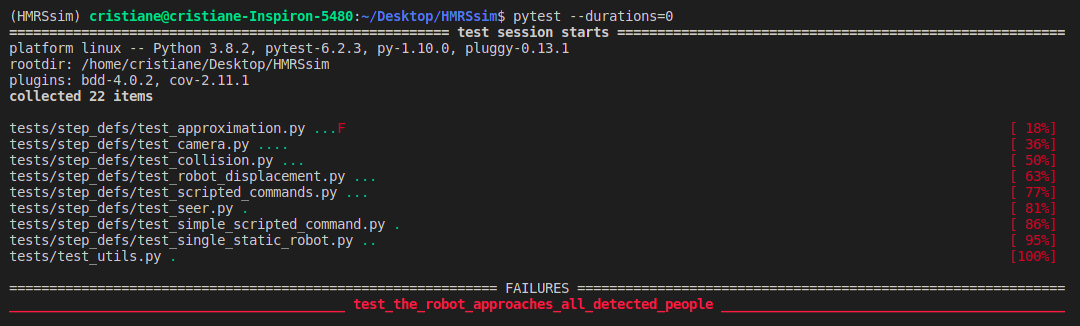
\includegraphics[width=\textwidth]{imagens/testResults.png}
\caption{Resultados do pytest.} 
\label{fig:testResults}
\end{figure}

\begin{figure}
\centering
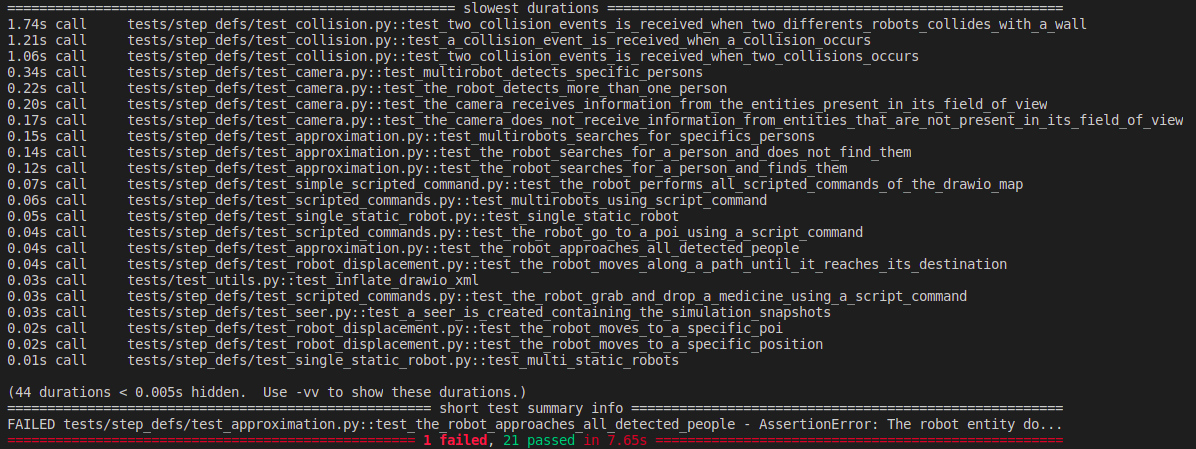
\includegraphics[width=\textwidth]{imagens/timeResults.png}
\caption{Resultados de tempo de execução do pytest.} 
\label{fig:timeResults}
\end{figure}

A figura \ref{fig:testResults} mostra o resultado da execução do pytest para todos os cenários citados abaixo. Pela imagem pode-se observar que todos os cenários estão passando, com exceção do último cenário do test\_approximation.py. Em relação a falha desse teste, uma observação pode ser feita: é possível detectar várias pessoas, conforme mostra o último cenário da \textit{feature Camera}, mas só é possível fazer uma aproximação, que será feita até a primeira entidade detectada.

Um ponto que pode ser observado é o tempo gasto para executar os testes da colisão, que é o maior de todos, conforme mostra a figura \ref{fig:timeResults}.

Da forma que o cenário foi implementado, o robô sai de um ponto inicial e se movimenta por um caminho determinado até colidir com a parede. O robô fica parado nessa parede até o final da simulação e durante todo esse tempo são enviados eventos dizendo que está ocorrendo a colisão.

O sistema de colisão (CollisionProcessor) é um sistema mais custoso que fica ativo durante toda a simulação verificando se ocorreu colisões entre as entidades. Para cada entidade que possui os componentes Collidable, Position, Velocity é verificado se ocorreu uma colisão com cada uma das outras entidades do mapa que possuem os componentes Collidable, Position, ou seja, é uma interação dentro de outra interação. No entanto, o que está causando o gargalo não é essa interação, mas sim a função collide, que é responsável por verificar se uma forma está colidindo com outra. Essa função é chamada dentro de outra função, a checkCollide (simulator/systems/CollisionProcessor.py). Para tentar diminuir o tempo de execução, algumas modificações foram feitas pelo Giovanni (como citar ele?). A imagem X, mostra o tempo de execução após as mudanças feitas no sistema de colisão.

\begin{figure}
\centering
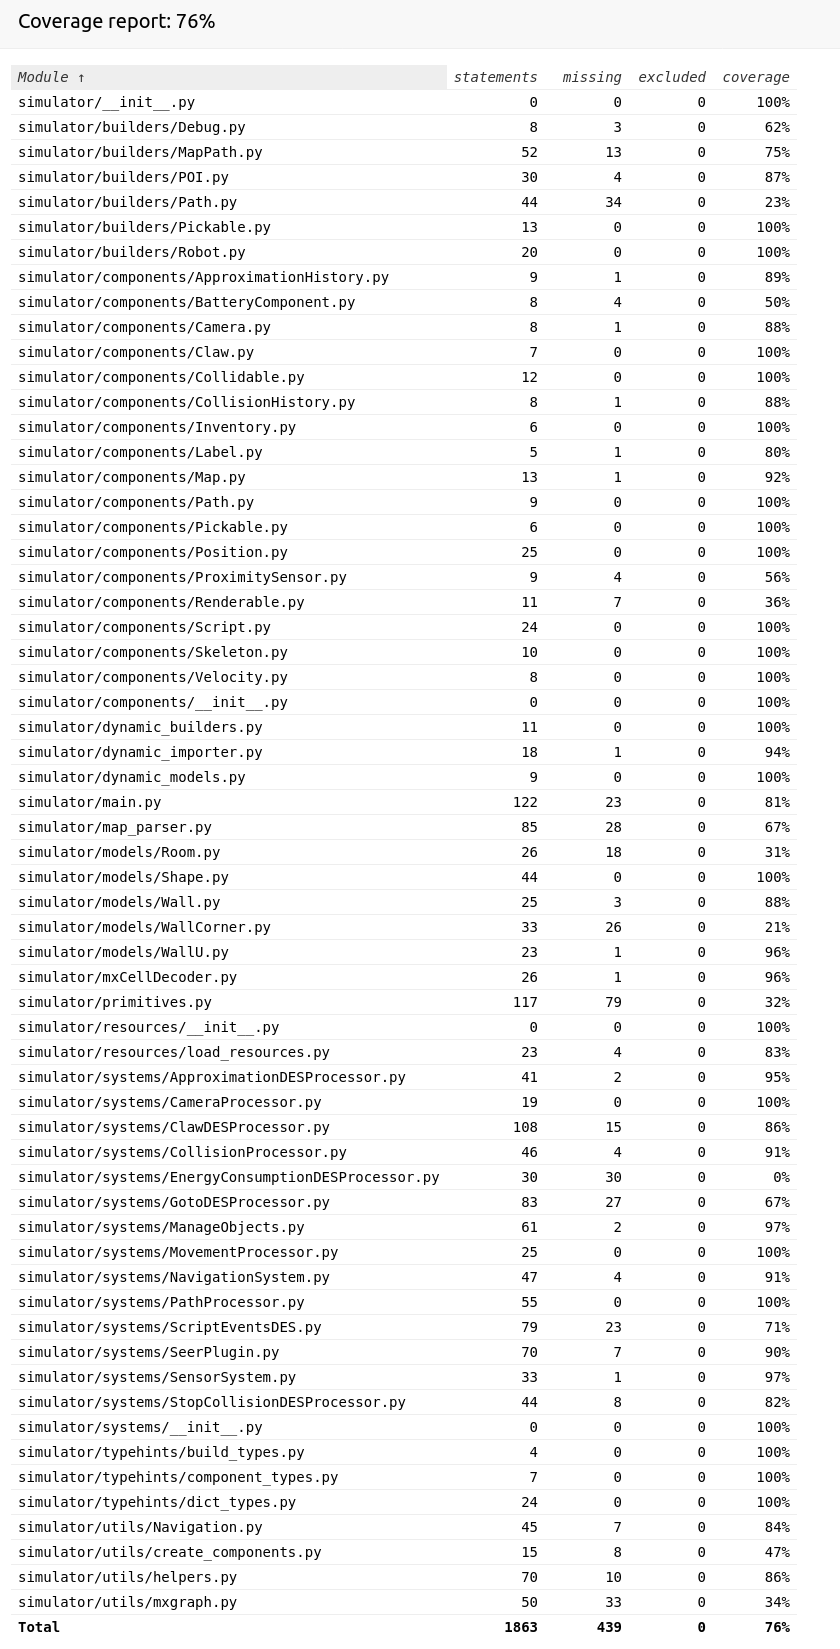
\includegraphics[scale=0.4]{imagens/coverage.png}
\caption{Cobertura dos testes.} 
\label{fig:coverage}
\end{figure}

A cobertura total dos testes ficou em 76\%, conforme mostra a figura \ref{fig:coverage}.
O sistema EnergyConsumptionDESProcessor está com a cobertura em 0\% porque ainda não foi terminado e não possui nenhum cenário de teste. No entanto, o sistema tem potencial e pode ser continuado em trabalhos futuros.

No geral, os cenários de teste usam todas as principais funcionalidades do sistema, conforme mostrado pelo coverage.

\subsection{Single Static Robot}
\label{sec:singleStaticRobot}
É composto por dois cenários. No primeiro cenário (Single static robot), o robô com id ‘robot’ está em uma posição 1,1 no mapa e ao executar a simulação, esse robô deve permanecer parado, pois não foi enviada nenhuma instrução para o robô se movimentar. Portanto, no final, o robô deve estar na posição 1,1.

O segundo cenário (Multi static robots) conta com multi-robôs, cada um numa posição diferente e todos esses robôs devem permanecer parados até o final da execução, pois nenhuma instrução foi dada.

Todos os dois cenários passam, pois todos os robôs permanecem na mesma posição, conforme o esperado.

\subsection{Simple Scripted Command}
\label{sec:simpleScriptedCommand}
É composto por um cenário (the robot performs all scripted commands of the drawio map) no qual o robô lê uma lista de comandos que foram adicionados a ele pelo edit data no drawio: [["Go medRoom", "Grab medicine", "Go patientRoom", "Drop medicine"], 0]. É esperado que o robô vá até a sala de medicamentos (medRoom), pegue o medicamento ‘medicine’ presente nesta sala e depois vá até a o quarto do paciente (pacientRoom) e deixe este medicamente lá. 

O teste passa para esse cenário, pois o robô segue todo o caminho esperado e deixa o medicamento no local correto.

\subsection{Scripted Commands}
\label{sec:scriptedCommands}
O teste é composto por três cenários. No primeiro (The robot Go to a POI using a script command) é verificado se o robô foi até o quarto de medicamentos usando o comando Go. No segundo (The robot grab and drop a medicine using a script command) é verificado se o robô deixou o medicamento no quarto do paciente utilizando os comandos Grab e Drop. No terceiro cenário (Multi-robots using script command) é testado se dois robôs realizam determinados comandos de forma paralela, o primeiro robô deixa um medicamento no quarto do paciente e o segundo robô vai até o quarto do paciente. Os cenários descritos utilizam o sistema de comandos (ScriptEventDES.py) e os comandos Go, Grab e Drop.

Os testes estão passando para todos os cenários descritos acima, pois os robôs seguem corretamente todos os comandos solicitados.

\subsection{Robot Displacement}
\label{sec:robotDisplacement}
O teste é composto por três cenários, no qual cada cenário descreve uma forma diferente de se locomover. Utilizando cada uma dessas três formas, o robô deve parar no mesmo ponto. No primeiro cenário (The robot moves along a path until it reaches its destination), a locomoção é feita através de uma seta (type: Path) que sai do robô e vai até um determinado destino. No segundo cenário (The robot moves to a specific Position), o robô recebe um comando para ir até uma posição (x, y). Já no terceiro cenário (The robot moves to a specific POI), o robô recebe um comando para se locomover até um POI (ponto de interesse).

Os três testes passam, pois o robô para no mesmo ponto de destino independente da forma de locomoção e da rota utilizada.

\subsection{Collision}
\label{sec:collision}
Existem três cenários para testar colisões simples. No primeiro cenário (A collision event is received when a collision occurs), o robô colide com uma parede e recebe uma notificação da ocorrência da colisão. No segundo cenário (Two collision events is received when two collisions occurs), o robô colide com duas paredes diferentes e recebe a notificação da ocorrência das duas colisões. No terceiro cenário (Two collision events is received when two differents robots collides with a wall), é testado se dois robôs colidem com uma parede e se  recebem a notificação de colisões de forma separada.

Todos os testes passam, pois os robôs recebem a notificação da colisão com a parede.

\subsection{Camera}
\label{sec:camera}
O teste é composto por quatro cenários. O primeiro cenário (The camera receives information from the entities present in its field of view) é responsável por  testar se a câmera detectou uma determinada entidade que estava no campo de visão dela. O segundo cenário (The camera does not receive information from entities that are not present in its field of view) é responsável  por testar se não foi detectada uma determinada entidade que não estava no campo de visão da câmera do robô. O terceiro cenário (Multi-robot detects specific persons) é responsável por testar se multi-robôs detectaram determinadas entidades que estavam em seu campo de visão. Já o último cenário (The robot detects more than one person) é responsável por verificar se um robô é capaz de detectar mais de uma pessoa que esteja em seu campo de visão.

Todos os testes passam, pois só são detectadas as entidades que estão no campo de visão da câmera e a funcionalidade serve para um cenário com multi-robôs.

\subsection{Approximation}
\label{sec:approximation}
O teste é composto por quatro cenários. No primeiro cenário (The robot searches for a person and finds them), o robô procura por uma pessoa usando uma câmera e assim que essa pessoa é detectada, o robô se aproxima dela. No segundo cenário (The robot searches for a person and does not find them), o robô procura por uma pessoa, mas não a encontra e logo, ele não se aproxima dela. No terceiro cenário (Multi-robots searches for specifics persons), é testado se mais de um robô com a capacidade de detectar outras entidades, se aproximam das entidades detectadas. No último cenário (The robot approaches all detected people), o robô procura por duas pessoas que estão no campo de visão dele e tenta se aproximar delas.

Os três primeiros testes passam, pois os robôs só se aproximam das entidades detectadas. Já o último teste falha, pois da forma que ocorreu a implementação do ApproximationDESProcessor só é possível fazer uma aproximação.

\subsection{Seer}
\label{sec:seer}
Foi feito um cenário básico (A seer is created containing the simulation snapshots) para testar o funcionamento do sistema Seer, que é responsável por obter snapshots da simulação. O teste cria um cenário simples de movimentação e adiciona o Seer para obter os snapshots. Os resultados obtidos serão salvos em um arquivo seer\_report.txt e depois será verificado se esse arquivo gerado contém os logs. No momento, para testar se o arquivo está correto, é verificado se a primeira linha dele possui um dicionário com uma chave chamada timestamp.

O teste feito passa,  pois o snapshot é gerado corretamente pelo sistema do Seer.

\section{Comparar os problemas apontados e como você tentou resolver eles}
\label{sec:problemasApontados}
Um dos problemas relatados pelos desenvolvedores que utilizam simuladores é a mudança constante nas APIs e a falta de documentação, principalmente em relação a essas mudanças.

Este problema também foi observado durante o desenvolvimento dos testes do HMRS sim e ocorria da seguinte forma: Era gasto um certo tempo para entender como funcionavam todos os parâmetros, sistemas e componentes necessários para fazer funcionar um determinado sistema e depois de entender o funcionamento, eram feitos os testes e eles passavam. No entanto, como a ferramenta estava em constante mudanças, quase toda vez que ocorria um pull da branch dev, todos os testes quebravam por conta de mudanças na forma que eram chamados determinados métodos (mudanças na API). Depois de quebrar os testes, era necessário procurar essas mudanças e os erros que estavam acontecendo para refazer os testes. 

As mudanças constantes na API causaram bastante retrabalho. O que ajudou bastante nessa parte foi que o desenvolvedor da ferramenta sempre ajudava quando entrava em contato com ele, caso contrário, não seria possível aplicar o bdd no projeto.

O que teria ajudado e o que pode ajudar em trabalhos futuros: 
\begin{itemize}
    \item Ter uma interface mais fixa ou ter uma comunicação mais clara da ocorrência de mudanças na interface.
    \item Executar os testes antes de dar um commit.
    \item Uma documentação mais completa e atualizada com todas as mudanças feitas na interface.
\end{itemize}

Outro problema relatado pelos desenvolvedores é não ser possível executar os testes sem desabilitar a Interface Gráfica. Também foi observado este problema no desenvolvimento de testes do HMR Sim quando a parte gráfica era acoplada com o restante do código. Quando estava acoplado, foi gasto semanas e esforço tentando construir os testes e mesmo assim não foi possível, principalmente por causa de dificuldades ao configurar a simulação e executar com a parte gráfica, sendo que uma das dificuldades relatadas é saber a hora de término da execução e fechar o simulador sem ser de forma manual.

Os testes começaram a serem feitos quando ocorreu a separação da parte gráfica do restante do código, assim foi possível verificar de forma mais simples diferentes variáveis e informações da simulação somente pelo código. Se não tivesse ocorrido essa separação, também não teria sido viável fazer a automação dos testes.

Outros aspectos que eram apontados pelos desenvolvedores como um problema era a dificuldade de executar a simulação sem intervenção manual e não ter uma terminação clara da simulação. No entanto, a arquitetura do simulador desenvolvido permite que a simulação funcione sem ser necessário a interação manual com uma interface gráfica e a simulação segue um número de passos limitados, sendo possível saber quando ela termina. Dessa forma, o HMR sim não possui esses dois problemas relatados e isso acaba facilitando a construção de testes e a automação deles.

A dificuldade na construção de cenários e ambientes também foi um problema relatado. Para contornar essa dificuldade foi proposto e desenvolvido um conjunto de métodos auxiliares para auxiliar na construção dos cenários e na realização das assertivas.

